\chapter{Webapp}\label{cap:webapp}

\section{Scopo del sistema}

La webapp permette all'utente di avere un interfaccia grafica con la quale gestire e monitorare lampioni, sensori ed aree, inoltre permette di visualizzarne le informazioni relative.

\section{Requisiti coperti dal sistema}

\subsection{RV\_01}
RV\_01: l'applicazione deve essere visualizzabile su dispositivi mobile.

\subsection{RV\_02}
RV\_02: l'applicazione client deve poter essere utilizzata sulla versione più recente di Chrome (v. 110.0).

\subsection{RV\_03}
RV\_03: l'applicazione client deve poter essere utilizzata sulla versione più recente di Firefox (v. 110.0).

\subsection{RV\_04}
RV\_04: l'applicazione client deve poter essere utilizzata sulla versione più recente di Safari (v. 16.3).

\subsection{RV\_05}
RV\_05: l'applicazione client deve essere conforme almeno al livello AA delle WCAG.


\section{Descrizione del sistema}

La webapp è stata sviluppata utilizzando il framework Angular, il quale permette di creare applicazioni web single-page e di gestire le dipendenze tra le varie componenti dell'applicazione. Inoltre, è stato utilizzato il framework Bootstrap per la gestione della parte grafica. L'applicazione utilizza componenti di Angular, servizi e chiamate API per comunicare con il server. Le principali features dell'applicazione sono:
\begin{itemize}
    \item Visualizzazione lista di lampioni, sensori ed aree;
    \item Cambiare lo status dei lampioni e dei sensori;
    \item Aggiungere lampioni, sensori ed aree;
    \item Gestire caricamenti ed errori durante le chiamate API;
    \item Implementare l'autenticazione;
    \item Proteggere i collegamenti all'applicazione; 
\end{itemize} 

\section{Architettura del sistema}

La classe Model implementa tre interfacce che definiscono lo status di lampioni,sensori ed aree, queste definiscono la struttura e forniscono le proprietà per immagazinare informazioni quali status, identificativo e alias. Le tre interfacce sono:
\begin{itemize}
    \item \textbf{LampStatus:} definisce lo stato di un lampione;
    \item \textbf{SensorStatus:} definisce lo stato di un sensore;
    \item \textbf{AreaStatus:} definisce lo stato di un'area;
\end{itemize}

\subsection{Servizi}

\begin{figure}[h]
    \centering
    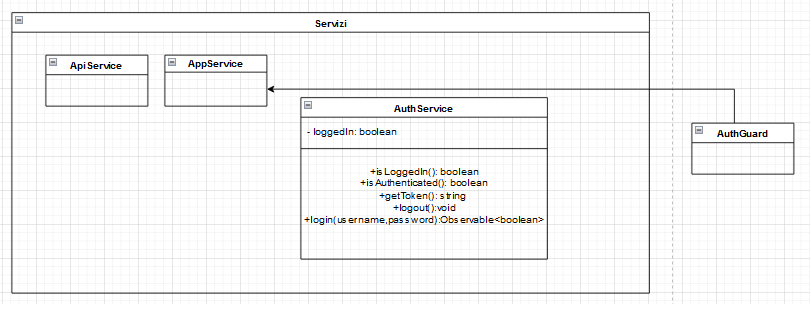
\includegraphics[width=\textwidth]{img/services_webapp.png}
    \caption{Servizi della webapp \ref{fig:services_webapp}}
    \label{fig:services_webapp}
\end{figure}

La classe \textbf{Apiservice} definisce i metodi per effettuare le chiamate API e interagire con il server, questo servizio mette a dispozione i metodi per:
\begin{itemize}
    \item Ottenere la lista di lampioni, sensori ed aree;
    \item Ottenere lo stato di un lampione, sensore o area;
    \item Modificare lo stato di un lampione, sensore o area;
    \item Aggiungere un lampione, sensore o area;
    \item Ottenere i dati di un sensore;
    \item Ottenere i dati di un'area;
\end{itemize}

L'applicazione presenta delle classi per l'utilizzo di altri microservizi:
\begin{itemize}
    \item \textbf{AuthService:} controlla l'autenticazione dell'utente;
    \item \textbf{AppService:} gestisce lo stato dell'applicazione mantenedo lo status di lampioni, sensori ed aree, questo servizio fornisce i metodi per l'aggiunta di nuovi dispositivi e comunica con l'API per ottenere dati, aggiornare gli status e gestire caricamenti ed errori;
\end{itemize}

La classe \textbf{AuthGuard} permette di proteggere i collegamenti all'applicazione, in questo modo l'utente non autenticato non può accedere alle pagine dell'applicazione.

\subsection{Componenti}

\begin{figure}[h]
    \centering
    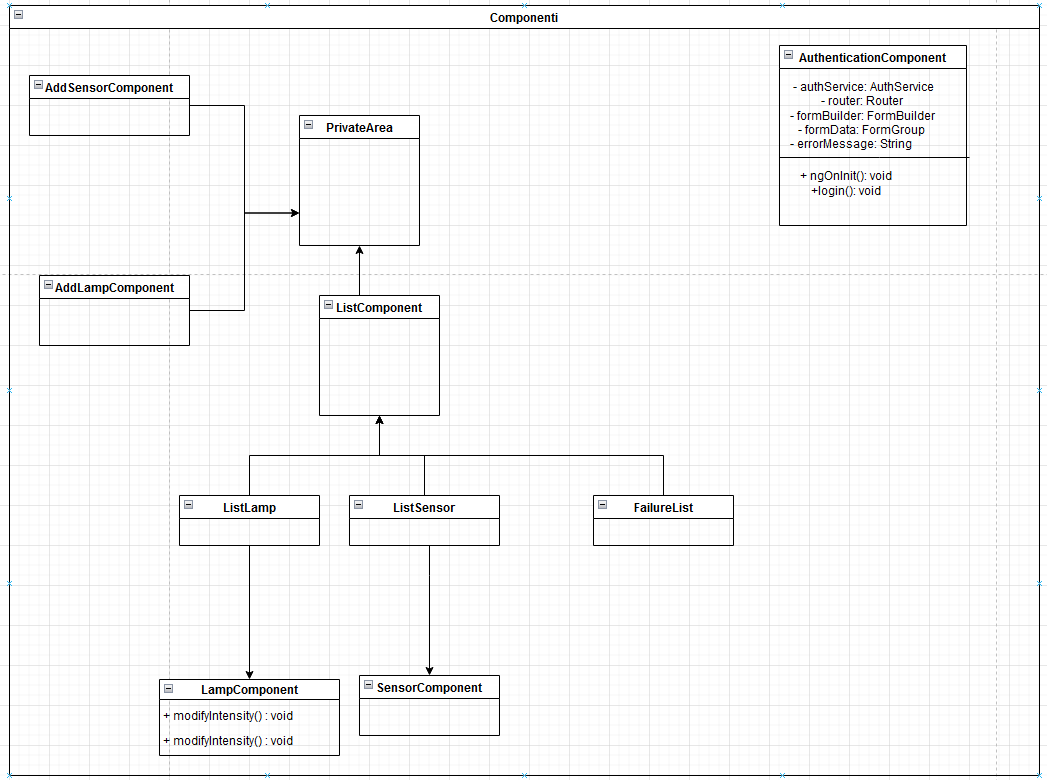
\includegraphics[width=\textwidth]{img/components_webapp.png}
    \caption{Componenti della webapp \ref{fig:components_webapp}}
    \label{fig:components_webapp}
\end{figure}

L'applicazione utilizza dei componenti per definire e gestire le varie parti dell'applicazione, questi sono:
\begin{itemize}
    \item \textbf{lamp.component:} rappresenta un lampione con il proprio stato e permette di modificarlo;
    \item \textbf{sensor.component:} rappresenta un sensore con il proprio stato e permette di modificarlo;
    \item \textbf{area.component:} rappresenta un'area di illuminazione;
    \item \textbf{lamps-list.component:} visualizza la lista di lampioni;
    \item \textbf{sensors-list.component:} visualizza la lista di sensori;
    \item \textbf{areas-list.component:} visualizza la lista di aree;
    \item \textbf{authentication.component:} gestitsce l'autenticazione dell'utente;
    \item \textbf{private-area.component:} gestisce l'area privata;
\end{itemize}